\documentclass[margin,line]{resume}
 
\usepackage{polyglossia}
\setdefaultlanguage[variant=us]{english}
\usepackage[none]{hyphenat}
\usepackage{graphicx,wrapfig}
\usepackage{url}
\usepackage{fontspec}
\usepackage{xltxtra}
\setmainfont{Minion Pro}
\usepackage[activate={true,nocompatibility},final,factor=1100,stretch=10,shrink=10,expansion=false,verbose=silent]{microtype}
\usepackage[colorlinks=true, pdfstartview=FitV,
linkcolor=blue, citecolor=blue, urlcolor=blue]{hyperref}
\frenchspacing
 
\begin{document}
\raggedright%
{\sc \Large Curriculum Vitae~---~Martin Bjeldbak Madsen}
\begin{resume}
    \vspace{0.5cm}
    \begin{wrapfigure}{4}{0.4\textwidth}
         \vspace{-1cm}
        \begin{center}
        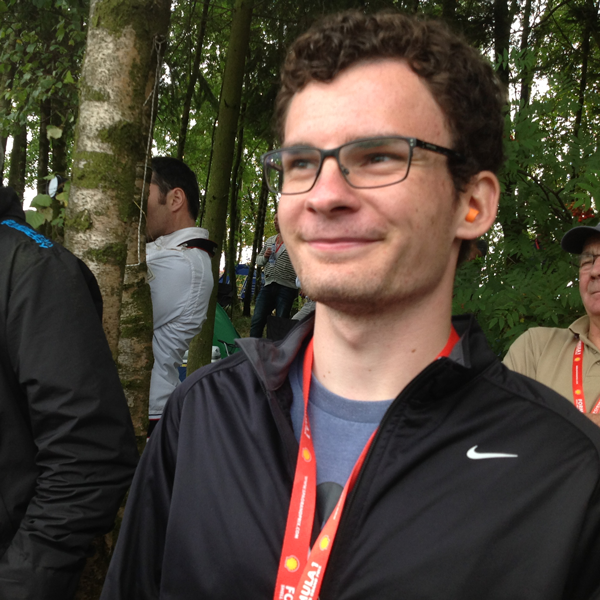
\includegraphics[width=0.4\textwidth]{moi.png}
        \end{center}
         \vspace{-3.5cm}
    \end{wrapfigure}

\section{\mysidestyle{} Personal\\Information}%\vspace{2mm}
    Martin Bjeldbak Madsen\\
    June 9th, 1992 (22 years old)\\ 
    3971 Haines St., Apt A\\
    92109 San Diego, CA \\
    Phone: (951) 249--2631\\
    \href{mailto:martinbmadsen@gmail.com}{martinbmadsen@gmail.com}\\
    \href{http://martinbmadsen.dk}{martinbmadsen.dk}\\
    \vspace{0.5cm}
    \href{http://dk.linkedin.com/in/martinbmadsen/}{linkedin.com/in/martinbmadsen}\\
    \href{https://github.com/martinbmadsen}{github.com/martinbmadsen}\\
    \href{https://keybase.io/martinb}{keybase.io/martinb}\\
    \href{https://twitter.com/fapper}{twitter.com/fapper}

    Hello there! My name's Martin and I was born and raised in Denmark until I was 5 years of age, whereafter my family moved for a total of 9 years abroad, 4 of which were spent in England, and 5 in the US\@. That means that I've learned English and Danish speaking with locals, and I can quickly adapt to new cultural environments.

    Currently I'm taking the first year of my masters degree in Computer Science from Aalborg University abroad at the University of California, San Diego. I sincerely hope my CV piques your interest.

    The final project of my bachelors degree in computer science from Aalborg University involved measuring diversity amongst artificial neural networks used in evolutionary algorithms to train neural networks. We are in the process of getting the article published.
    
    %I've had a Danish driver's license for 4 years.
    I hold Danish and American driver's licenses.

\section{\mysidestyle{} Education}
    \textbf{University of California, San Diego~---~Computer Science}
    (2014--2015) Taking graduate level courses in Computer Science in connection with the first of my master's degree from Aalborg University.

    \textbf{Aalborg University~---~Master of Science, Computer Science}
    (2014--2016) Working on a master's degree in Computer Science, studying abroad the first year.

    \textbf{Aalborg University~---~Bachelor of Science, Computer Sience}
    (2011--2014) Bachelor's degree in Computer Science (180 ECTS credits). I graduated with an average of B on the European ECTS scale.      

    \textbf{EUC Nord~---~HTX} (2008--2011) Technical gymnasium in Hjørring, Denmark. I took the highest level Math, Physics, English, Electronics, and Danish possible.
    
    \textbf{Bagterpskolen} (2006--2008) Danish Folkeskole Education in Hjørring, Denmark.

    \textbf{J.\ R.\ Gerrits Middle School} (2003--2006) Kimberly, Wisconsin, USA\@.

\section{\mysidestyle{} Professional\\experience}\vspace{1mm}
\begin{description}

  \item[September 2012 $\rightarrow$ September 2014] Student software developer at Falck (30k employees) in their Falck Healthcare subsidiary. I developed new features and maintained a Rails web application used daily by around 40 of Falck's physiotherapists to journal their patients' developments. I was in constant contact with the physiotherapists, listening to their feedback and, acting and implementing features to enable them to more efficiently get their job done.

  \item[Sept 2010 $\rightarrow$ January 2014] Ran my own company,
  \emph{Divambu}. I developed and hosted web sites for small companies.

  \item[October 2008 $\rightarrow$ June 2010] Service worker at Fakta
  a/s (part of Coop Danmark, 36k employees). I was in direct contact
  with customers and fulfilled everyday tasks required to run a busy
  grocery store. I worked during evenings, weekends, and holidays
  alongside attending school full-time while I was under 18.
\end{description}

\section{\mysidestyle{} Other activities}\vspace{1mm}
\begin{description}
  \item[July 2012 $\rightarrow$ March 2014] Mentor, Project
    \href{http://www.urk.dk/solskinsunge/}{Solskinsunge} 2012. Volenteer
    work, where we arranged bi-monthly social gatherings for teenagers aged
    15--18, most of which are second generation immigrants.

  \item[January 2013 $\rightarrow$ September 2014] Elected student member of the
  Study Board of Computer Science at Aalborg University. The Study Board
  consists of 5 students and 5 professors, representing the student body
  and faculty groups. Here, we took on responsibilities
  for undergraduate and graduate programs within the Computer Science
  group and their curricular. We discussed, among others, qualification
  and exemption aplications, quality assurance, etc.
\end{description}

\section{\mysidestyle{} Skills} \vspace{1mm}
I love learning new techniques, methods, and tools, but there are a few technologies and systems I have more experience with than others:
\vspace{0.5cm}
\begin{description}
  \item[Operating systems] Intermediate understanding of most Unix-like systems: Ubuntu, Debian, CentOS, Arch Linux, Mac OS X.
  \item[Servers and databases] Nginx, Postgres, MySQL\@.
  \item[CMS-systems] I've set up systems with Wordpress, phpBB, Octopress.
  \item[Revision control] Git, SVN\@.
  \item[Programming, scripting, and markup languages] \LaTeX\ and \XeTeX, HTML, CSS, C, C$\sharp$, Java, JavaScript and jQuery, Ruby and Ruby on Rails. Currently learning: Haskell, Swift.
\end{description}

\section{\mysidestyle{} Language}
My native language is Danish, but almost everything I write and read is in English.

\begin{description}
  \item[Danish] mother tongue
  \item[Spoken English] fluent
  \item[Written English] fluent 
\end{description}

\section{\mysidestyle{} Interests}
I love to tea culture and reading books of all types. As far as sports go, I only follow Formula 1. Also, I enjoy working on small projects of my own to help broaden my interests and knowledge, such as toying with iOS apps, or working on a web app in a new technology. Keeping my body healthy and in shape is also important to me, as I believe it keeps my mind fit and open, too.

%There is also nothing better than traveling the world, so I try to do that as much as possible, and thankfully due to my fantastic friends, I've had quite a few amazing experiences traveling to visit them. I also enjoy electronic and classical music. 
\end{resume}
\end{document}
